\subsection{Sequence Diagram}

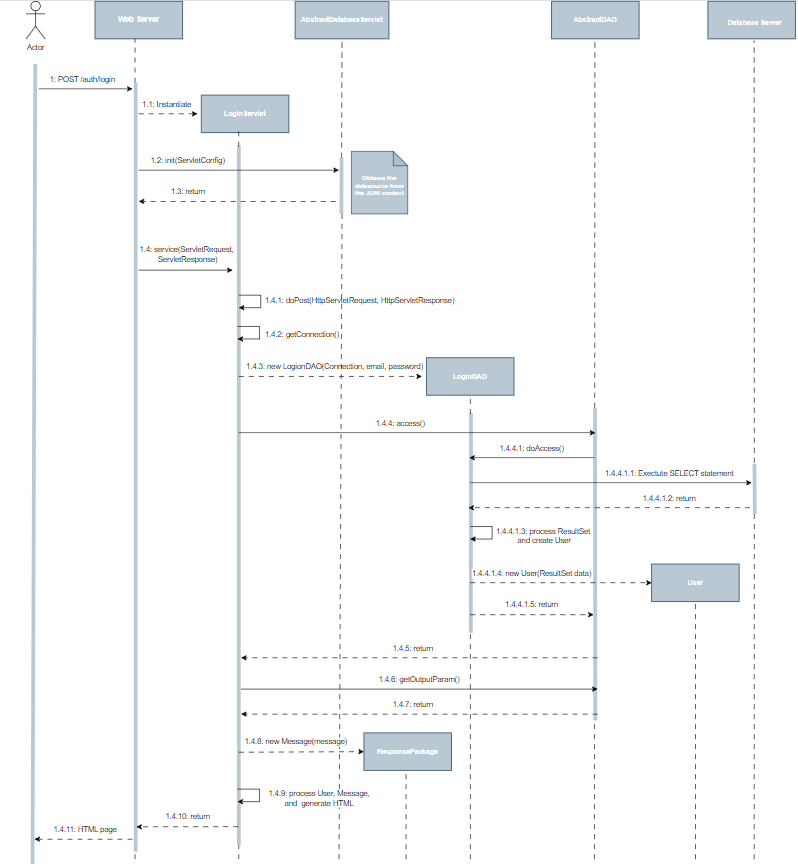
\includegraphics[scale = 0.8]{sections/BLL/sequenceDiagram.png}

Here is reported the sequence diagram for the operation about the login of a simple user. The user initiates the login process by sending a POST request to the web server.
The web server instantiates the LoginServlet and gets the
information about the datasource from the init method of the AbstractDatabaseServlet. 
After that it calls the doPost() method of the LoginServlet, passing the HttpServletRequest and the HTTPServletResponse. 
The LoginServlet analyzes the request and recognizes that it is a SELECT operation,indicating a login attempt, thus it
verifies the user's credentials using the request parameters. 
After that, a ResponsePackage is used to encapsulate the response from the API, providing a structured format for conveying the response status and message, along with any associated data.
In the end, the UserServlet replies to the web server, indicating the outcome of the login process using methods like setStatus() and getWriter(), which notify whether the operation was successful or not.


\textbf{ALTERNATIVE}
This sequence diagram shows the login operation. The operation is instantiated when an actor executes a POST request with a login credentials to the web server. The web server instantiates the LoginServlet and gets the information about the datasource from the AbstractDatabaseServlet. After that it calls the doPost method of the LoginServlet, passing the HttpServletRequest and the HTTPServletResponse. The LoginServlet then passes the Connection and login credentials to LoginDAO which executes SELECT statement on the database in order to check if the User with the credentials exists. After that, the LoginServlet replies to the web server with the appropriate response and HTML page.